% !TEX root = main.tex

\section{Graph-based inertial-kinematic odometry}

We describe the inertial-kinematic odometry for legged robots, based on a graph model. 

\subsection{Graph-based estimation through non-linear least squares optimization}

Estimation is realized with a tool in ongoing development \textbf{(cite WOLF ?)} and using Google Ceres non-linear least squares optimizer. This optimization is run on data given by the front-end part of the framework,
which aim is to formalize the problem according to the graph-based model for aforementioned reasons. This representation, illustrated in \figRef{fig:factor_graph}, 
gives a human-readable way to easily visualize optimized states (circles) linked to constraining information during the optimization process (factors drawn as squares). Constraints are set by the front-end process using measurements from sensors.
Thus, it is possible to constrain states with several factors provided by different sensors leading to a fusion. Factor play a key role since they are used on top of previous states to predict next ones and compute the error with the current states.
The optimal states are computed so that the overall residual is minimized in a least squares meaning.

\subsection{The inertial-kinematic odometry}
\subsubsection{Inertial pre-integration}
\subsubsection{Graphical model}

\begin{figure}[tb]
\begin{center}
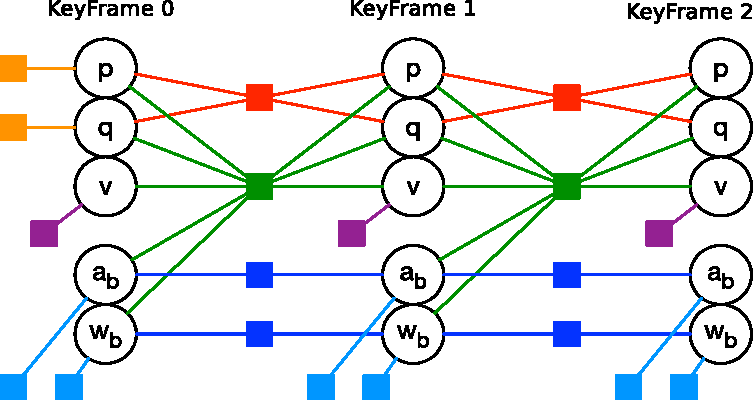
\includegraphics[scale=0.65]{figures/graph_exploded}
%\par\vspace{4mm}
%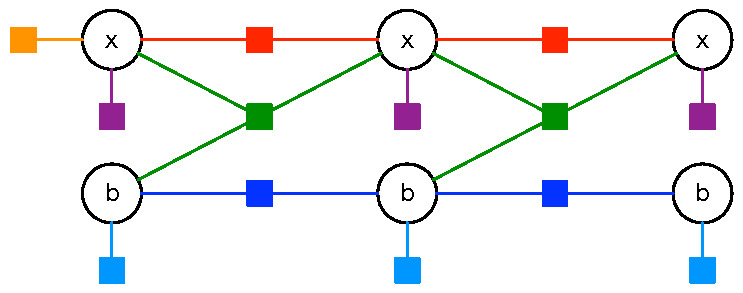
\includegraphics[scale=0.65]{figures/graph_simplified}
\par\vspace{4mm}
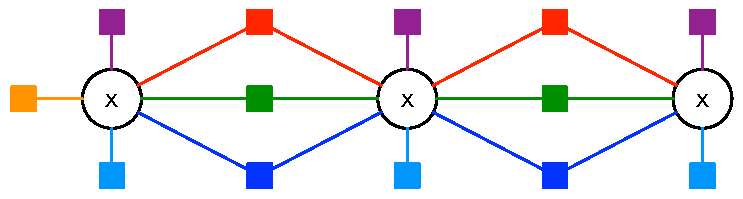
\includegraphics[scale=0.65]{figures/graph_essential}
\caption{
{\bf Top}: Detailed factor graph for the initial keyframe and two steps. \emph{Circles}: state blocks for position ($p$), orientation quaternion ($q$), velocity ($v$), accelerometer bias ($a_b$), gyrometer bias ($\omega_b$). \emph{Orange}: initial pose factor. \emph{Red}: leg kinematic factor. \emph{Green}: IMU's delta pre-integration factor. 
\emph{Blue}: bias drift factor. \emph{Cyan}: bias absolute factor. \emph{Purple}: zero-velocity factor. 
%{\bf Mid}: Simplified factor graph where aggregate state blocks $x=(p,q,v)$ and biases $b=(a_b,\omega_b)$ are used. 
{\bf Bottom}: Equivalent factor graph exhibiting one aggregate state block $x=(p,q,v,a_b,\omega_b)$ for each key-frame. All factors are affecting exactly the same variables as in the Top graph.
}
\label{fig:factor_graph}
\end{center}
\end{figure}

%\begin{figure}[htbp]
%\begin{center}
%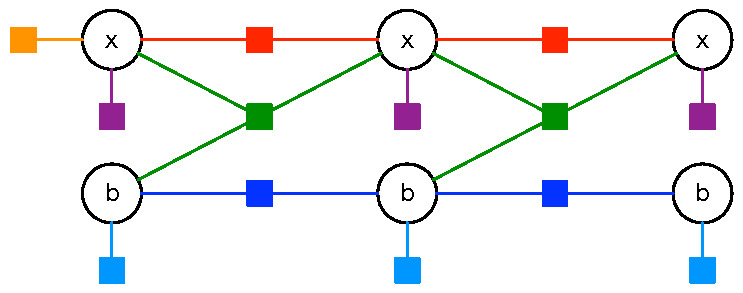
\includegraphics[scale=0.65]{figures/graph_simplified}
%\caption{default}
%\label{default}
%\end{center}
%\end{figure}

